\documentclass[10pt,a4paper]{article}
\usepackage[utf8]{inputenc}
\usepackage[T1]{fontenc}
\usepackage[margin=0.85in,top=1in,bottom=0.9in]{geometry}
\usepackage{amsmath,amssymb}
\usepackage{booktabs,longtable,tabularx,array}
\usepackage{xcolor}
\usepackage{tikz}
\usetikzlibrary{arrows.meta,positioning}
\usepackage{enumitem}
\usepackage{listings}
\usepackage{titlesec}
\usepackage{fancyhdr}
\usepackage[most]{tcolorbox}
\usepackage[colorlinks=true,linkcolor=secondary,urlcolor=secondary]{hyperref}

\definecolor{primary}{RGB}{18,52,86}
\definecolor{secondary}{RGB}{0,102,204}
\definecolor{codebg}{RGB}{245,247,250}
\definecolor{rulegray}{RGB}{200,208,218}

\setlength{\parindent}{0pt}
\sloppy\setlength{\emergencystretch}{4em}
\setlength{\parskip}{0.5em}
\setlist{itemsep=0.2em,topsep=0.3em,parsep=0pt}
\renewcommand{\arraystretch}{1.25}

\pagestyle{fancy}
\fancyhf{}
\renewcommand{\headrulewidth}{0.4pt}
\lhead{\color{gray}\small Wholesale Supermarket Management System}
\rhead{\color{gray}\small Group 23 | IIT (BHU) CSE}
\rfoot{\thepage}

\titleformat{\section}{\Large\bfseries\color{primary}}{\thesection}{0.8em}{}[\color{rulegray}\titlerule]
\titleformat{\subsection}{\large\bfseries\color{secondary}}{\thesubsection}{0.8em}{}
\titleformat{\subsubsection}{\normalsize\bfseries\color{primary}}{\thesubsubsection}{0.8em}{}
\titlespacing*{\section}{0pt}{1.6em}{0.6em}

\newcommand{\code}[1]{\texttt{\detokenize{#1}}}
\newtcolorbox{note}[1][Note]{colback=secondary!6,colframe=secondary,fonttitle=\bfseries,title=#1,boxrule=0.5pt,arc=2pt,left=6pt,right=6pt,top=4pt,bottom=4pt,breakable}
\newtcolorbox{warnbox}[1][Heads-up]{colback=orange!8,colframe=orange!80!black,fonttitle=\bfseries,title=#1,boxrule=0.5pt,arc=2pt,left=6pt,right=6pt,top=4pt,bottom=4pt,breakable}
\newtcolorbox{qbox}[1]{colback=white,colframe=primary,fonttitle=\bfseries\small,title={#1},boxrule=0.5pt,arc=2pt,left=6pt,right=6pt,top=4pt,bottom=4pt,breakable}

\lstdefinestyle{base}{
  basicstyle=\ttfamily\footnotesize,
  backgroundcolor=\color{codebg},
  frame=single, rulecolor=\color{rulegray},
  breaklines=true, breakatwhitespace=false,
  keywordstyle=\color{secondary}\bfseries,
  commentstyle=\color{gray}\itshape,
  stringstyle=\color{teal},
  xleftmargin=4pt, xrightmargin=4pt, aboveskip=0.6em, belowskip=0.4em,
  columns=fullflexible, keepspaces=true, showstringspaces=false
}
\lstset{style=base}
\lstdefinelanguage{SQLx}{
  morekeywords={CREATE,VIEW,AS,SELECT,FROM,JOIN,LEFT,ON,GROUP,BY,WHERE,FOR,UPDATE,CHECK,PROCEDURE,IN,OUT,BEGIN,END,DECLARE,DEFAULT,INSERT,INTO,VALUES,SET,IF,THEN,LEAVE,START,TRANSACTION,COMMIT,ROLLBACK,DELIMITER,EXIT,HANDLER,SQLEXCEPTION,AND,IS,NOT,NULL,DECIMAL,INT,VARCHAR,JSON,CAST,COALESCE,SUM,ROUND,GREATEST,CONCAT,FLOOR,LIKE,ENUM,TABLE},
  sensitive=false, morecomment=[l]{--}, morestring=[b]'}

\begin{document}

\begin{titlepage}
\centering
\vspace*{2.2cm}
{\color{primary}\rule{\textwidth}{1.2pt}}\\[1.2em]
{\Huge\bfseries\color{primary} Wholesale Supermarket\\[0.3em] Management System}\\[0.8em]
{\Large\color{secondary} Master Project \& Viva Guide}\\[1.2em]
{\color{primary}\rule{\textwidth}{1.2pt}}\\[2.5em]
{\large Course: Database Management Systems (CS321 / DBMS Lab)}\\[0.4em]
{\large Department of Computer Science \& Engineering\\ Indian Institute of Technology (BHU), Varanasi}\\[1.4em]
{\Large\bfseries Group 23}\\[2em]
\begin{tabular}{rl}
\textbf{Domain:} & FMCG \& commodity wholesale (Muzaffarnagar, UP)\\
\textbf{Database:} & MySQL 8.0 (InnoDB)\\
\textbf{Backend:} & Python 3.14, FastAPI, PyMySQL, JWT, Passlib (bcrypt)\\
\textbf{Frontend:} & Semantic HTML5, CSS, ES6 vanilla JavaScript\\
\textbf{Academic Year:} & 2026
\end{tabular}
\vfill
{\small\color{gray} Written so that every team member can understand and defend the whole project.}
\end{titlepage}

\tableofcontents
\newpage

%--------------------------------------------------------------
\section{Executive Summary \& Business Context}
\subsection{The business problem}
Standard retail Point of Sale (POS) software fails for wholesale agricultural and commodity trading. A wholesale dealer in Muzaffarnagar (Western UP) deals with four product categories:
\begin{itemize}
  \item \textbf{Kriyana} (groceries and grains): Basmati rice, refined sugar, mustard oil, spices.
  \item \textbf{Dryfruits:} almonds, cashews, pistachios, raisins.
  \item \textbf{Desi Jadi Booti} (herbal / Ayurvedic commodities): ashwagandha roots, dried tulsi leaves, mulethi.
  \item \textbf{Tota Rang Gulal:} Holi colours and herbal gulal pigments.
\end{itemize}

\subsection{Core wholesale challenges and how we answer them}
\begin{longtable}{@{}p{3.0cm}p{6.0cm}p{6.5cm}@{}}
\toprule
\textbf{Challenge} & \textbf{Why it matters} & \textbf{Our design answer}\\
\midrule\endhead
Price volatility & Prices change batch by batch with mandi arrivals; one item can have several batches bought at different rates. & Price lives in \code{Batch}, not \code{Item}.\\
Perishability & Spices, dryfruits and herbs expire; dead stock is a direct loss. & FEFO allocation (First-Expired, First-Out) using \code{Expiry_Date}.\\
GST compliance & Rates of 0\%, 5\%, 12\%, 18\%; intra-state sales split 50/50 into CGST and SGST with HSN codes on the invoice. & Insert-only \code{HSN_Tax_Rate} table; split computed in views.\\
Audit-proof financials & Stored totals drift when quantities or rates change (update anomalies). & Bill totals and line taxes are \textbf{never stored}; they are derived by views.\\
Concurrency & Many cashiers bill at once; the last 10 kg of cashews must not be sold twice. & Transactions with \code{SELECT ... FOR UPDATE} row locks.\\
\bottomrule
\end{longtable}

\subsection{System at a glance}
\begin{itemize}
  \item 3-tier architecture: browser UI $\rightarrow$ FastAPI REST API $\rightarrow$ MySQL 8.0.
  \item 14 normalized tables (3NF/BCNF) and 13 views.
  \item Stored procedure \code{sp_create_bill}: atomic FEFO billing with loyalty handling.
  \item Three roles: \textbf{Owner}, \textbf{Employee} (cashier), \textbf{Customer}, with JWT-based RBAC.
\end{itemize}

%--------------------------------------------------------------
\section{High-Level System Architecture}
\begin{center}
\resizebox{\textwidth}{!}{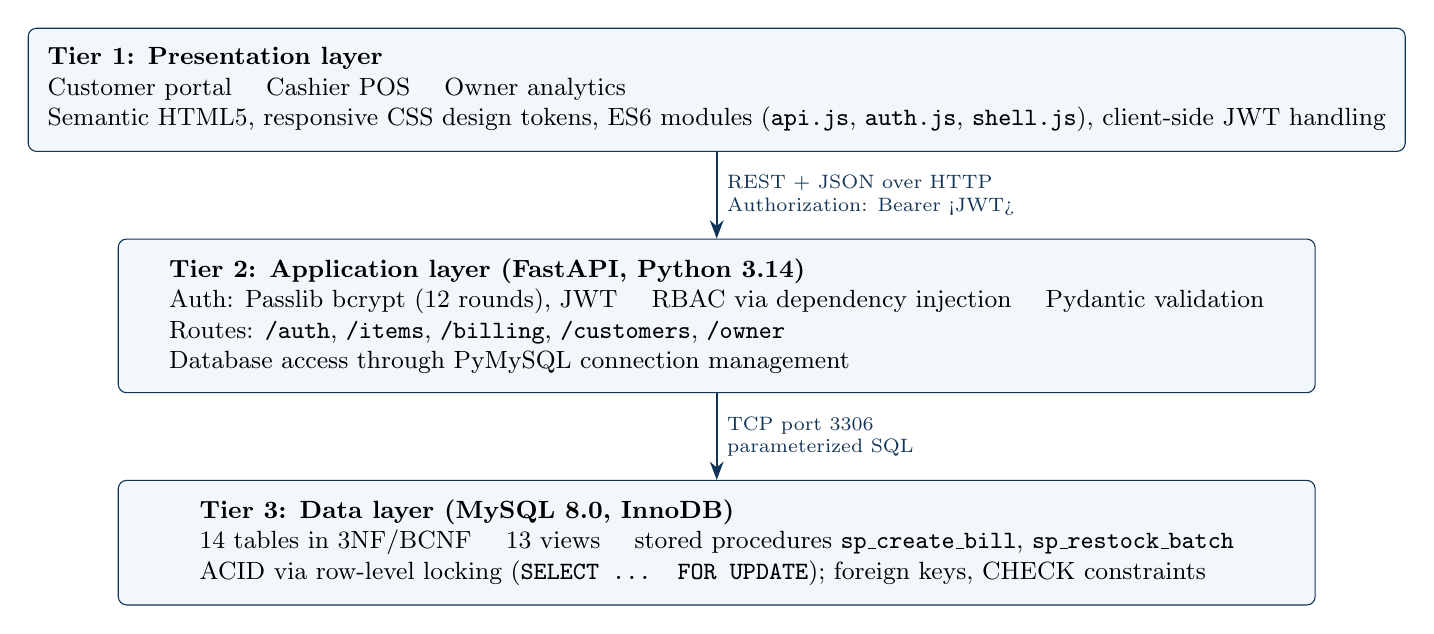
\begin{tikzpicture}[node distance=0.7cm,
  tier/.style={draw=primary,fill=secondary!5,rounded corners=3pt,minimum width=15.2cm,align=left,inner sep=7pt,font=\small},
  arr/.style={-{Stealth},thick,color=primary}]
\node[tier] (t1) {\textbf{Tier 1: Presentation layer}\\
Customer portal \quad Cashier POS \quad Owner analytics\\
Semantic HTML5, responsive CSS design tokens, ES6 modules (\texttt{api.js}, \texttt{auth.js}, \texttt{shell.js}), client-side JWT handling};
\node[tier,below=1.1cm of t1] (t2) {\textbf{Tier 2: Application layer (FastAPI, Python 3.14)}\\
Auth: Passlib bcrypt (12 rounds), JWT \quad RBAC via dependency injection \quad Pydantic validation\\
Routes: \texttt{/auth}, \texttt{/items}, \texttt{/billing}, \texttt{/customers}, \texttt{/owner}\\
Database access through PyMySQL connection management};
\node[tier,below=1.1cm of t2] (t3) {\textbf{Tier 3: Data layer (MySQL 8.0, InnoDB)}\\
14 tables in 3NF/BCNF \quad 13 views \quad stored procedures \texttt{sp\_create\_bill}, \texttt{sp\_restock\_batch}\\
ACID via row-level locking (\texttt{SELECT ... FOR UPDATE}); foreign keys, CHECK constraints};
\draw[arr] (t1) -- node[right,font=\scriptsize,align=left]{REST + JSON over HTTP\\Authorization: Bearer <JWT>} (t2);
\draw[arr] (t2) -- node[right,font=\scriptsize,align=left]{TCP port 3306\\parameterized SQL} (t3);
\end{tikzpicture}}
\end{center}

\subsection{Why this stack (viva justification)}
\begin{itemize}
  \item \textbf{MySQL 8.0 InnoDB:} real ACID transactions, row-level locking, views, CHECK constraints.
  \item \textbf{FastAPI:} asynchronous, automatic OpenAPI/Swagger docs at \code{/docs}, strong typing via Pydantic, dependency-injected security.
  \item \textbf{Vanilla ES6 modules:} no Node.js, webpack or npm; the frontend runs directly in the browser and is easy to debug.
\end{itemize}

%--------------------------------------------------------------
\section{Repository \& Codebase Anatomy}
\begin{lstlisting}[basicstyle=\ttfamily\scriptsize]
DBMSProject/
+-- db/
|   +-- 01_schema.sql       # 14 tables, PKs, FKs, CHECKs, indexes
|   +-- 02_views.sql        # 13 views (financial, inventory, analytics)
|   +-- 03_seed.sql         # realistic Muzaffarnagar wholesale seed data
|   +-- 04_procedures.sql   # sp_create_bill, sp_restock_batch
+-- app/
|   +-- main.py             # FastAPI entrypoint, CORS, route registration
|   +-- database.py         # MySQL connection pool and cursor management
|   +-- services/auth_service.py   # bcrypt hashing, JWT, RBAC guards
|   +-- routes/
|       +-- auth_routes.py       # login, profile
|       +-- item_routes.py       # catalog, categories, batches
|       +-- billing_routes.py    # POS checkout, invoices
|       +-- customer_routes.py   # portal, requests, feedback, loyalty
|       +-- owner_routes.py      # BI reports, inventory, employees
+-- frontend/               # served by FastAPI under /app
|   +-- index.html          # landing / login
|   +-- customer/  staff/  owner/   # role-specific pages
|   +-- js/                 # api.js, auth.js, shell.js, ui.js
|   +-- css/                # tokens.css, base.css, layout.css, components.css
+-- tests/
|   +-- test_concurrency.py # multi-threaded proof of row locking
|   +-- test_loyalty.py     # loyalty calculation and limit tests
|   +-- test_schema.py      # schema invariants and views
+-- DEMO.md  ER_DIAGRAM.md  PROJECT_MASTER_GUIDE.md/.pdf  requirements.txt
\end{lstlisting}

%--------------------------------------------------------------
\section{Relational Database Schema (14 Tables)}
The database \code{supermarket_db} has 14 tables normalized to 3NF/BCNF.

\subsection{Summary of keys and constraints}
\begin{longtable}{@{}p{3.0cm}p{3.1cm}p{9.5cm}@{}}
\toprule
\textbf{Table} & \textbf{Primary key} & \textbf{Foreign keys / key constraints}\\
\midrule\endhead
1. Category & \code{Category_ID} & UNIQUE(\code{Category_Name})\\
2. Supplier & \code{Supplier_ID} & UNIQUE(\code{Phone_Number}), UNIQUE(\code{GSTIN})\\
3. HSN\_Tax\_Rate & \code{HSN_Code} & Insert-only; \code{Tax_Rate} in percent (0, 5, 12, 18)\\
4. Item & \code{Item_ID} & FK $\to$ Category; UNIQUE(\code{Item_Name})\\
5. Batch & \code{Batch_ID} & FK $\to$ Item, Supplier, HSN\_Tax\_Rate; CHECK(\code{Live_Stock >= 0})\\
6. Customer & \code{Customer_ID} & UNIQUE(\code{Phone_Number}); CHECK(\code{Loyalty_Points >= 0})\\
7. Employee & \code{Employee_ID} & UNIQUE(\code{Phone_Number}), UNIQUE(\code{Aadhaar_Number})\\
8. Users & \code{User_ID} & UNIQUE(\code{Username}); FK $\to$ Employee, Customer; Role ENUM(Owner, Employee, Customer)\\
9. Bill & \code{Bill_ID} & FK $\to$ Customer (NULL for walk-ins), FK $\to$ Employee (\code{Billed_By_Employee_ID})\\
10. Bill\_Details & (\code{Bill_ID}, \code{Batch_ID}) & Composite PK; FK $\to$ Bill, Batch; CHECK(\code{Quantity > 0})\\
11. Stock\_Request & \code{Request_ID} & FK $\to$ Customer, Item, Employee; XOR CHECK on item reference\\
12. Loyalty\_Transaction & \code{Transaction_ID} & FK $\to$ Customer, Bill; \code{Points_Change} is signed\\
13. Feedback & \code{Feedback_ID} & FK $\to$ Customer, Bill; CHECK(\code{Rating BETWEEN 1 AND 5})\\
14. Settings & \code{Setting_Key} & Key-value system configuration\\
\bottomrule
\end{longtable}

\subsection{Table definitions}
\subsubsection*{1. Category}
Top-level commodity groups. \code{Category_ID} (INT, AUTO\_INCREMENT, PK); \code{Category_Name} (VARCHAR(50), NOT NULL, UNIQUE); \code{Description} (TEXT).

\subsubsection*{2. Supplier}
Wholesale vendors. \code{Supplier_ID} (PK); \code{Supplier_Name} (VARCHAR(100), NOT NULL); \code{Contact_Person}; \code{Phone_Number} (VARCHAR(15), NOT NULL, UNIQUE); \code{Email}; \code{Address} (TEXT); \code{GSTIN} (VARCHAR(15), UNIQUE; the 15-character GST identification number).

\subsubsection*{3. HSN\_Tax\_Rate (insert-only)}
\code{HSN_Code} (VARCHAR(10), PK); \code{Tax_Rate} (DECIMAL(5,2), NOT NULL, CHECK $\ge 0$); \code{Description}; \code{Effective_From} (DATE, NOT NULL).
\begin{note}[Architectural rule]
This table is strictly \textbf{insert-only}. When the government changes a rate, a new row is inserted; existing rows are never updated or deleted. This preserves historical billing integrity.
\end{note}

\subsubsection*{4. Item}
The abstract product (for example ``Basmati Rice 1121''). \code{Item_ID} (PK); \code{Item_Name} (NOT NULL, UNIQUE); \code{Category_ID} (FK, NOT NULL); \code{Unit} (e.g.\ kg, litre, packet); \code{Reorder_Level} (INT, default 10).
\textbf{Item holds no price and no tax rate;} those belong to \code{Batch}.

\subsubsection*{5. Batch}
A physical stock lot arriving at the godown. \code{Batch_ID} (PK); \code{Item_ID}, \code{Supplier_ID}, \code{HSN_Code} (all FK, NOT NULL); \code{Batch_Number}; \code{Purchase_Price} (cost from supplier); \code{Wholesale_Price} (selling price, tax-exclusive); \code{Initial_Stock} (CHECK $\ge 0$); \code{Live_Stock} (CHECK $\ge 0$, decremented on sale); \code{Received_Date}; \code{Expiry_Date} (drives FEFO); \code{Is_Active} (BOOLEAN, default TRUE).

\subsubsection*{6. Customer}
\code{Customer_ID} (PK); \code{Customer_Name}; \code{Phone_Number} (UNIQUE); \code{Email}; \code{Address}; \code{GSTIN} (optional, for B2B buyers); \code{Loyalty_Points} (INT, default 0, CHECK $\ge 0$; running balance).

\subsubsection*{7. Employee}
\code{Employee_ID} (PK); \code{First_Name}; \code{Last_Name}; \code{Phone_Number} (UNIQUE); \code{Email}; \code{Role} (Cashier, Manager, Store Staff); \code{Salary}; \code{Aadhaar_Number} (VARCHAR(12), UNIQUE); \code{Is_Active}.

\subsubsection*{8. Users}
Authentication and RBAC. \code{User_ID} (PK); \code{Username} (UNIQUE); \code{Password_Hash} (VARCHAR(255), bcrypt, 12 rounds); \code{Role} ENUM(Owner, Employee, Customer); \code{Employee_ID} and \code{Customer_ID} (nullable FKs); \code{Last_Login}; \code{Is_Active}.

\subsubsection*{9. Bill}
Invoice header. \code{Bill_ID} (PK); \code{Bill_Number} (UNIQUE); \code{Customer_ID} (nullable FK; NULL means walk-in); \code{Billed_By_Employee_ID} (FK, NOT NULL); \code{Bill_Date} (DATETIME, default now); \code{Payment_Method} ENUM(Cash, UPI, Card, Credit); \code{Loyalty_Points_Redeemed} (CHECK $\ge 0$).
\textbf{Subtotal, GST and net amount are not stored here;} they are computed in \code{v_bill_totals}.

\subsubsection*{10. Bill\_Details}
Invoice line items: \code{Bill_ID}, \code{Batch_ID}, \code{Quantity} (CHECK $> 0$), PRIMARY KEY (\code{Bill_ID}, \code{Batch_ID}). The unit price is \emph{not} duplicated; it is joined from \code{Batch.Wholesale_Price}.

\subsubsection*{11. Stock\_Request}
Demand-driven procurement requests. \code{Request_ID} (PK); \code{Customer_ID} (FK); \code{Item_ID} (nullable FK, for restocking an existing item); \code{Requested_Item_Name} (nullable, for a brand-new product); \code{Quantity_Requested} (CHECK $> 0$); \code{Request_Date}; \code{Status} ENUM(Pending, Approved, Rejected, Fulfilled); \code{Remarks}; \code{Handled_By_Employee_ID} (nullable FK).
\begin{lstlisting}[language=SQLx]
CHECK ((Item_ID IS NOT NULL) <> (Requested_Item_Name IS NOT NULL))
\end{lstlisting}
A request names \emph{either} an existing item \emph{or} a new item, never both and never neither (exclusive OR).

\subsubsection*{12. Loyalty\_Transaction}
Immutable audit ledger of reward points: \code{Transaction_ID} (PK); \code{Customer_ID}; \code{Bill_ID} (nullable); \code{Points_Change} (positive when earned, negative when redeemed); \code{Transaction_Date}; \code{Reason}.

\subsubsection*{13. Feedback}
\code{Feedback_ID} (PK); \code{Customer_ID}; \code{Bill_ID}; \code{Rating} (TINYINT, 1 to 5); \code{Comments}; \code{Created_At}.

\subsubsection*{14. Settings}
\code{Setting_Key} (PK); \code{Setting_Value}; \code{Description}. Key parameters: \code{Loyalty_Earn_Rate} (100.00), \code{Loyalty_Redeem_Rate} (1.00), \code{Loyalty_Max_Discount_Percent} (50.00).

%--------------------------------------------------------------
\section{Relational Views (13 Views)}
Views give abstraction, enforce business rules and avoid redundant stored data.

\subsection{Financial views}
\textbf{1.\ \code{v_bill_lines}} computes price, GST rate, CGST, SGST and total for each bill line.
\begin{lstlisting}[language=SQLx]
CREATE VIEW v_bill_lines AS
SELECT bd.Bill_ID, bd.Batch_ID, i.Item_Name, b.Batch_Number, bd.Quantity,
  b.Wholesale_Price AS Unit_Price,
  (bd.Quantity * b.Wholesale_Price) AS Line_Subtotal,
  htr.Tax_Rate AS GST_Rate,
  ROUND((bd.Quantity * b.Wholesale_Price) * (htr.Tax_Rate / 100.0) / 2.0, 2) AS CGST_Amount,
  ROUND((bd.Quantity * b.Wholesale_Price) * (htr.Tax_Rate / 100.0) / 2.0, 2) AS SGST_Amount,
  ROUND((bd.Quantity * b.Wholesale_Price) * (1.0 + htr.Tax_Rate / 100.0), 2) AS Line_Total
FROM Bill_Details bd
JOIN Batch b ON bd.Batch_ID = b.Batch_ID
JOIN Item i ON b.Item_ID = i.Item_ID
JOIN HSN_Tax_Rate htr ON b.HSN_Code = htr.HSN_Code;
\end{lstlisting}

\textbf{2.\ \code{v_bill_totals}} aggregates the lines into the fiscal summary of each bill.
\begin{lstlisting}[language=SQLx]
CREATE VIEW v_bill_totals AS
SELECT b.Bill_ID, b.Bill_Number, b.Bill_Date, b.Customer_ID, c.Customer_Name,
  b.Billed_By_Employee_ID,
  CONCAT(e.First_Name, ' ', e.Last_Name) AS Cashier_Name,
  b.Payment_Method, b.Loyalty_Points_Redeemed,
  CAST(b.Loyalty_Points_Redeemed AS DECIMAL(10,2)) AS Loyalty_Discount,
  COALESCE(SUM(vbl.Line_Subtotal), 0.00) AS Subtotal,
  COALESCE(SUM(vbl.CGST_Amount), 0.00) AS CGST_Total,
  COALESCE(SUM(vbl.SGST_Amount), 0.00) AS SGST_Total,
  COALESCE(SUM(vbl.CGST_Amount + vbl.SGST_Amount), 0.00) AS GST_Total,
  COALESCE(SUM(vbl.Line_Total), 0.00) AS Gross_Amount,
  GREATEST(0.00, COALESCE(SUM(vbl.Line_Total), 0.00)
    - CAST(b.Loyalty_Points_Redeemed AS DECIMAL(10,2))) AS Net_Payable
FROM Bill b
LEFT JOIN Customer c ON b.Customer_ID = c.Customer_ID
JOIN Employee e ON b.Billed_By_Employee_ID = e.Employee_ID
LEFT JOIN v_bill_lines vbl ON b.Bill_ID = vbl.Bill_ID
GROUP BY b.Bill_ID;
\end{lstlisting}

\subsection{Inventory views}
\begin{itemize}
  \item \textbf{3.\ \code{v_active_batches}:} batches available for sale (\code{Live_Stock > 0} and \code{Expiry_Date >= CURDATE()}).
  \item \textbf{4.\ \code{v_expiring_batches}:} batches expiring within 30 days, for promotions.
  \item \textbf{5.\ \code{v_low_stock}:} total active stock per item compared with \code{Reorder_Level}.
  \item \textbf{6.\ \code{v_stock_summary}:} units on hand and capital tied up per item.
\end{itemize}

\subsection{Business intelligence views}
\begin{itemize}
  \item \textbf{7.\ \code{v_daily_sales}:} daily revenue, bill counts and tax collected.
  \item \textbf{8.\ \code{v_monthly_sales}:} monthly trends for reporting.
  \item \textbf{9.\ \code{v_category_sales}:} revenue per commodity category.
  \item \textbf{10.\ \code{v_top_selling_items}:} items ranked by quantity and revenue.
  \item \textbf{11.\ \code{v_customer_summary}:} lifetime value, order count, loyalty balance.
  \item \textbf{12.\ \code{v_supplier_purchases}:} acquisition cost per supplier.
  \item \textbf{13.\ \code{v_gst_summary}:} CGST and SGST collected per HSN class (tax reconciliation).
\end{itemize}

%--------------------------------------------------------------
\section{Formal Normalization Analysis (1NF to BCNF)}
\begin{center}
\resizebox{\textwidth}{!}{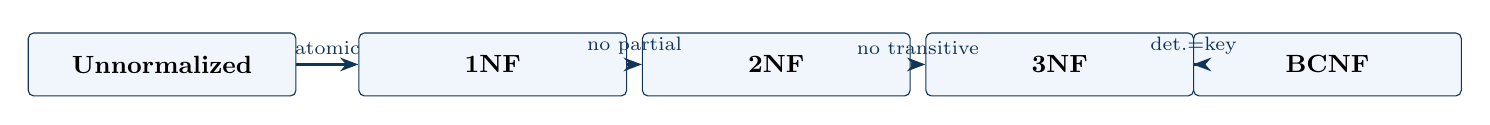
\begin{tikzpicture}[box/.style={draw=primary,fill=secondary!6,rounded corners=2pt,minimum width=3.4cm,minimum height=0.8cm,font=\small\bfseries,align=center},
  a/.style={-{Stealth},thick,color=primary},lab/.style={font=\scriptsize,align=left}]
\node[box] (u) at (0,0) {Unnormalized};
\node[box] (n1) at (4.2,0) {1NF};
\node[box] (n2) at (7.8,0) {2NF};
\node[box] (n3) at (11.4,0) {3NF};
\node[box] (bc) at (14.8,0) {BCNF};
\draw[a] (u)--(n1) node[midway,above,lab]{atomic};
\draw[a] (n1)--(n2) node[midway,above,lab]{no partial};
\draw[a] (n2)--(n3) node[midway,above,lab]{no transitive};
\draw[a] (n3)--(bc) node[midway,above,lab]{det.=key};
\end{tikzpicture}}
\end{center}

\subsection{First Normal Form (1NF)}
Every attribute holds atomic values; there are no repeating groups or comma-separated lists. Line items are decomposed into the junction table \code{Bill_Details} instead of being packed into a column of \code{Bill}.

\subsection{Second Normal Form (2NF)}
Must be in 1NF, and every non-prime attribute must depend on the \emph{whole} candidate key.
In \code{Bill_Details} the key is $(\text{Bill\_ID}, \text{Batch\_ID})$ and the only non-key attribute is \code{Quantity}:
\[ (\text{Bill\_ID}, \text{Batch\_ID}) \to \text{Quantity} \]
Neither attribute alone determines \code{Quantity}, so there is no partial dependency. \code{Item_Name}, \code{Wholesale_Price} and \code{Tax_Rate} are deliberately \emph{not} in \code{Bill_Details}; they would depend on \code{Batch_ID} alone (a partial dependency) and violate 2NF.

\subsection{Third Normal Form (3NF)}
Must be in 2NF, and no non-prime attribute may be transitively dependent on a key.
\begin{itemize}
  \item A flat design would have $\text{Batch\_ID} \to \text{HSN\_Code} \to \text{Tax\_Rate}$, a transitive dependency. We resolve it by moving the rate into its own relation \code{HSN_Tax_Rate(HSN_Code, Tax_Rate, ...)}; \code{Batch} keeps only the \code{HSN_Code} foreign key.
  \item \code{Item}: $\text{Item\_ID} \to (\text{Item\_Name}, \text{Category\_ID}, \text{Unit})$. \code{Batch}: $\text{Batch\_ID} \to (\text{Item\_ID}, \text{Supplier\_ID}, \text{HSN\_Code}, \text{Wholesale\_Price}, \dots)$.
  \item \textbf{Derivable attributes:} storing \code{Subtotal} or \code{Net_Amount} in \code{Bill} makes it depend on aggregated \code{Bill_Details} rows. Changing a quantity or a rate would leave the stored total inconsistent (an update anomaly). Computing totals in \code{v_bill_totals} avoids this.
\end{itemize}

\subsection{Boyce-Codd Normal Form (BCNF)}
For every non-trivial dependency $X \to Y$, $X$ must be a superkey. In all 14 tables, each determinant is either the primary key or a candidate key enforced by a UNIQUE index (e.g.\ \code{Supplier.Phone_Number}, \code{Users.Username}, \code{Customer.Phone_Number}). Hence the schema satisfies BCNF.

%--------------------------------------------------------------
\section{Transactions, Concurrency \& ACID}
\subsection{The ``last unit'' race condition}
Suppose 10 units of cashews remain and two cashiers bill 10 units simultaneously \emph{without} locking:
\begin{enumerate}
  \item Cashier 1 reads \code{Live_Stock = 10} (sufficient). Cashier 2 also reads 10 (sufficient).
  \item Both set \code{Live_Stock = 10 - 10 = 0}.
  \item Both print invoices: 20 units sold from 10 physical units.
\end{enumerate}
The result is overselling, an inventory deficit and a classic \textbf{lost update} anomaly.

\subsection{Solution: pessimistic row locking}
\begin{lstlisting}[language=SQLx]
SELECT Live_Stock, Expiry_Date
FROM Batch
WHERE Batch_ID = ?
FOR UPDATE;
\end{lstlisting}
\code{FOR UPDATE} takes an exclusive (X) lock on the batch row inside the transaction. Cashier 2's transaction waits until Cashier 1 issues \code{COMMIT} or \code{ROLLBACK}. When it resumes it reads \code{Live_Stock = 0}, detects insufficient stock and rejects the second bill.

\subsection{Verification: \texttt{tests/test\_concurrency.py}}
The test creates a batch with exactly 1 unit and starts 2 worker threads that check out concurrently. \textbf{Observed result:} exactly one thread succeeds (HTTP 200) and the other fails with HTTP 400 (\emph{Insufficient stock}). No double allocation occurs.

\subsection{ACID in this system}
\begin{longtable}{@{}p{2.2cm}p{13.4cm}@{}}
\toprule
\textbf{Property} & \textbf{Mechanism}\\
\midrule\endhead
Atomicity & Inserting \code{Bill} and \code{Bill_Details}, deducting \code{Live_Stock}, adjusting loyalty points and writing \code{Loyalty_Transaction} all happen in \emph{one} transaction. Any failure triggers \code{ROLLBACK}, leaving no orphan rows.\\
Consistency & The engine enforces CHECK (\code{Live_Stock >= 0}), foreign keys (\code{ON DELETE RESTRICT}) and the Stock\_Request XOR rule; violating transactions abort.\\
Isolation & InnoDB's default REPEATABLE READ (MVCC) plus explicit \code{SELECT ... FOR UPDATE} prevents dirty reads, non-repeatable reads and lost updates on inventory rows.\\
Durability & InnoDB write-ahead logging (redo log). After \code{COMMIT} the changes survive crashes and power loss.\\
\bottomrule
\end{longtable}

%--------------------------------------------------------------
\section{Stored Procedures \& FEFO Allocation}
\subsection{The FEFO algorithm}
When a cashier bills 25 kg of Basmati rice, several batches may exist:
\begin{itemize}
  \item Batch 101: 10 kg left, expires Dec 2026.
  \item Batch 102: 20 kg left, expires Mar 2027.
\end{itemize}
FEFO allocation: order active batches by \code{Expiry_Date ASC}; take 10 kg from Batch 101 (now 0) and the remaining 15 kg from Batch 102 (5 kg left); insert two \code{Bill_Details} rows, one per batch. Nothing near expiry is left unsold.

\subsection{\texttt{sp\_create\_bill}}
Located in \code{db/04_procedures.sql}; it wraps the whole checkout in one MySQL transaction. The FEFO loop (step 4) is summarized as a comment here.
\begin{lstlisting}[language=SQLx,basicstyle=\ttfamily\scriptsize]
DELIMITER //
CREATE PROCEDURE sp_create_bill(
  IN p_customer_id INT, IN p_employee_id INT, IN p_payment_method VARCHAR(20),
  IN p_redeem_points INT,
  IN p_items_json JSON,   -- [{"item_id": 1, "qty": 10}, ...]
  OUT p_bill_id INT, OUT p_status_message VARCHAR(255))
proc_body: BEGIN
  DECLARE v_bill_number VARCHAR(50);
  DECLARE v_net_total DECIMAL(10,2) DEFAULT 0.00;
  DECLARE v_earned_points INT DEFAULT 0;
  DECLARE v_cust_points INT DEFAULT 0;

  DECLARE EXIT HANDLER FOR SQLEXCEPTION
  BEGIN
    ROLLBACK;
    SET p_bill_id = NULL;
    SET p_status_message = 'Transaction rolled back due to error.';
  END;

  START TRANSACTION;
  -- 1. Validate loyalty points if redeeming (lock the customer row)
  IF p_customer_id IS NOT NULL AND p_redeem_points > 0 THEN
    SELECT Loyalty_Points INTO v_cust_points FROM Customer
    WHERE Customer_ID = p_customer_id FOR UPDATE;
    IF p_redeem_points > v_cust_points THEN
      ROLLBACK;
      SET p_bill_id = NULL;
      SET p_status_message = 'Cannot redeem more points than customer balance.';
      LEAVE proc_body;
    END IF;
  END IF;

  -- 2. Generate bill number
  SET v_bill_number = CONCAT('BILL-', DATE_FORMAT(NOW(), '%Y%m%d%H%i%s'));

  -- 3. Insert bill header
  INSERT INTO Bill (Bill_Number, Customer_ID, Billed_By_Employee_ID,
                    Payment_Method, Loyalty_Points_Redeemed)
  VALUES (v_bill_number, p_customer_id, p_employee_id, p_payment_method,
          COALESCE(p_redeem_points, 0));
  SET p_bill_id = LAST_INSERT_ID();

  -- 4. FEFO: iterate items, lock batches (FOR UPDATE), deduct stock,
  --    insert Bill_Details rows.   [loop omitted for brevity]

  -- 5. Earned points: 1 point per Rs 100 of net paid
  SELECT Net_Payable INTO v_net_total FROM v_bill_totals WHERE Bill_ID = p_bill_id;
  SET v_earned_points = FLOOR(v_net_total / 100);

  -- 6. Update loyalty ledger and balance
  IF p_customer_id IS NOT NULL THEN
    IF p_redeem_points > 0 THEN
      INSERT INTO Loyalty_Transaction (Customer_ID, Bill_ID, Points_Change, Reason)
      VALUES (p_customer_id, p_bill_id, -p_redeem_points, 'Redeemed at checkout');
    END IF;
    IF v_earned_points > 0 THEN
      INSERT INTO Loyalty_Transaction (Customer_ID, Bill_ID, Points_Change, Reason)
      VALUES (p_customer_id, p_bill_id, v_earned_points, 'Earned from purchase');
    END IF;
    UPDATE Customer
    SET Loyalty_Points = Loyalty_Points - COALESCE(p_redeem_points, 0) + v_earned_points
    WHERE Customer_ID = p_customer_id;
  END IF;

  COMMIT;
  SET p_status_message = 'Bill generated successfully.';
END //
DELIMITER ;
\end{lstlisting}

%--------------------------------------------------------------
\section{Core Business Logic \& Financial Accounting}
\subsection{Pricing and tax formulae}
Wholesale sales are priced tax-exclusive:
\begin{align*}
\text{Line Subtotal} &= \text{Quantity} \times \text{Wholesale Price}\\
\text{Line GST} &= \text{Line Subtotal} \times \tfrac{\text{GST Rate}}{100}\\
\text{CGST} = \text{SGST} &= \tfrac{\text{Line GST}}{2}\\
\text{Line Total} &= \text{Line Subtotal} + \text{Line GST}\\
\text{Gross Amount} &= \textstyle\sum \text{Line Total}\\
\text{Net Payable} &= \max\!\big(0,\ \text{Gross Amount} - \text{Loyalty Discount}\big)
\end{align*}

\subsection{Loyalty reward engine}
\begin{itemize}
  \item \textbf{Earn rate:} 1 point per Rs~100 of net amount paid.
  \item \textbf{Redemption:} 1 point = Rs~1 discount on the invoice.
  \item \textbf{Cap:} at most 50\% of the gross bill (protects dealer margin).
  \item \textbf{Walk-ins} (\code{Customer_ID = NULL}) neither earn nor redeem.
\end{itemize}
\textbf{Three-layer guard against over-redemption:}
\begin{enumerate}
  \item \textbf{UI:} the POS input is clamped to $\min(\text{balance},\ 50\%\text{ of gross})$.
  \item \textbf{API:} the FastAPI route compares points with the live balance and returns HTTP 400 if exceeded.
  \item \textbf{Database:} \code{sp_create_bill} locks the customer row, and rolls back with an error message if points exceed the balance.
\end{enumerate}

\subsection{Demand-driven stock requests}
Customers can request out-of-stock or unlisted products. The XOR constraint means \code{Item_ID} is set \emph{or} \code{Requested_Item_Name} is set. \textbf{Smart auto-matching:} if a customer types ``basmati rice'', the backend does a case-insensitive lookup, resolves it to the existing \code{Item_ID} and stores it as a catalog request.

%--------------------------------------------------------------
\section{Security Architecture \& Threat Defense}
\subsection{Password cryptography}
Passwords are never stored in plain text. We use bcrypt (via Passlib) with 12 cost rounds and a unique random 128-bit salt per password, which defeats rainbow tables; the cost factor deliberately slows brute force.

\subsection{Stateless authentication (JWT)}
\code{POST /auth/login} validates credentials and returns a signed JWT (HS256) that expires after 8 hours:
\begin{lstlisting}
{ "sub": "owner", "role": "Owner", "user_id": 1, "exp": 1793498400 }
\end{lstlisting}
Clients send it as \code{Authorization: Bearer <token>}.

\subsection{Role-based access control}
\begin{lstlisting}[language=Python,morekeywords={def,return,raise,if,not,in}]
def require_role(allowed_roles: list[str]):
    def dependency(token_data: dict = Depends(get_current_user)):
        if token_data["role"] not in allowed_roles:
            raise HTTPException(status_code=status.HTTP_403_FORBIDDEN,
                                detail="Access denied: Insufficient permissions.")
        return token_data
    return dependency
\end{lstlisting}
\begin{itemize}
  \item \code{/owner/*} requires \code{['Owner']}.
  \item \code{/billing/*} requires \code{['Owner', 'Employee']}.
  \item \code{/customers/me/*} requires \code{['Customer']}.
\end{itemize}

\subsection{SQL injection defense}
No raw string concatenation; every query is parameterized through PyMySQL:
\begin{lstlisting}[language=Python]
cursor.execute(
    "SELECT * FROM Item WHERE Item_Name LIKE %s AND Category_ID = %s",
    (f"%{query}%", category_id))
\end{lstlisting}
User input is sent separately from the SQL text and is treated purely as data.

%--------------------------------------------------------------
\section{Three-Role Operational Workflows}
\subsection{Customer portal}
\begin{itemize}
  \item \textbf{Dashboard} (\code{customer/home.html}): loyalty balance, profile, recent activity.
  \item \textbf{Catalog} (\code{catalog.html}): category filters, wholesale rates, stock badges (In stock, Low stock, Out of stock).
  \item \textbf{Stock requests} (\code{requests.html}): request restocks or suggest new commodities.
  \item \textbf{Invoices} (\code{bills.html}, \code{invoice.html}): past purchases and printable GST invoices with CGST/SGST breakdown.
  \item \textbf{Feedback} (\code{feedback.html}): 1 to 5 star rating with comments.
\end{itemize}
\subsection{Cashier POS terminal (\texttt{staff/pos.html})}
\begin{itemize}
  \item Customer phone lookup shows name and loyalty balance.
  \item Cart with live unit price, live stock validation and line subtotals.
  \item Payment methods: Cash, UPI, Card, Credit.
  \item Loyalty redemption with clamping and real-time balance check.
  \item One-click atomic checkout: creates the bill, deducts FEFO stock, updates loyalty, opens the printable invoice.
\end{itemize}
\subsection{Owner dashboard and BI}
\begin{itemize}
  \item \textbf{Dashboard:} KPIs (total bills, low stock, pending requests, expiring batches), 30-day revenue chart, top 5 items.
  \item \textbf{Inventory \& batches:} add incoming batches, adjust stock, track supplier lots.
  \item \textbf{Stock requests:} approve or reject customer requests.
  \item \textbf{Seven reports:} (1) sales trends, (2) category performance, (3) top-selling items, (4) low-stock alert, (5) expiring batches, (6) customer valuation, (7) GST tax summary.
\end{itemize}

%--------------------------------------------------------------
\section{Master Viva Grill: 25 Questions \& Model Answers}

\begin{qbox}{Q1. Why MySQL 8.0 rather than a NoSQL database like MongoDB?}
Wholesale trade needs financial accounting, stock deduction and statutory GST compliance, which demand ACID guarantees, referential integrity and joins. In a denormalized document store, updating an HSN rate or deducting stock atomically across concurrent cashiers needs complex application-level locking and risks lost updates. InnoDB gives row locking (\code{SELECT ... FOR UPDATE}), rollback, foreign keys and views natively.
\end{qbox}

\begin{qbox}{Q2. Why are Subtotal, GST and Total not stored in \texttt{Bill}?}
They are derivable attributes. Storing them creates a dependency on the aggregated lines, so a corrected quantity or changed rate would make the stored total diverge (update anomaly, a 3NF concern). \code{v_bill_totals} computes them on the fly from \code{Bill_Details}, \code{Batch} and \code{HSN_Tax_Rate}, so they are always consistent.
\end{qbox}

\begin{qbox}{Q3. Why is \texttt{HSN\_Tax\_Rate} insert-only?}
GST rates change by notification. If a rate were updated in place (say HSN 1006 from 5\% to 12\%), every historical bill would retroactively show 12\% through the views and falsify past filings. With insert-only rows, each batch keeps its foreign key to the rate valid when it was purchased, giving an unalterable audit trail.
\end{qbox}

\begin{qbox}{Q4. Explain the race condition on the last unit and your fix.}
Two cashiers both read \code{Live_Stock = 1}, both deduct, and two invoices are printed for one physical unit (lost update / double allocation). We run the deduction in a transaction with \code{SELECT Live_Stock FROM Batch WHERE Batch_ID = ? FOR UPDATE}, which takes an exclusive row lock. The second transaction waits, then reads 0, raises an error and the bill is rejected.
\end{qbox}

\begin{qbox}{Q5. Difference between 3NF and BCNF? Is your schema in BCNF?}
3NF: for every dependency $X \to Y$, either $X$ is a superkey or $Y$ is a prime attribute. BCNF removes the second exception: $X$ must always be a superkey. In our schema every determinant is a primary key or an enforced UNIQUE candidate key (e.g.\ \code{Phone_Number}, \code{Username}), so it is in BCNF.
\end{qbox}

\begin{qbox}{Q6. What is FEFO and why not FIFO?}
FIFO sells by arrival date; FEFO sells by \code{Expiry_Date ASC}. A newer batch can expire earlier because of harvest variation, so FEFO clears the stock nearest to expiry first and minimizes spoilage.
\end{qbox}

\begin{qbox}{Q7. How is the XOR constraint in \texttt{Stock\_Request} implemented?}
A request must reference an existing item or propose a new name, never both or neither. In MySQL 8: \code{CHECK ((Item_ID IS NOT NULL) <> (Requested_Item_Name IS NOT NULL))}. Each IS NOT NULL test yields 1 or 0, so \code{<>} is true exactly when the two differ, which is XOR.
\end{qbox}

\begin{qbox}{Q8. How do you stop a customer redeeming more points than they have?}
Three layers: the POS UI clamps the input to $\min(\text{points},\ 50\%\text{ of gross})$; the API (\code{billing_routes.py}) reads the live balance and returns HTTP 400 if exceeded; and \code{sp_create_bill} locks the customer row with \code{FOR UPDATE}, compares, and rolls back with an error message if the request is too large.
\end{qbox}

\begin{qbox}{Q9. Why split \texttt{Item} and \texttt{Batch}?}
One item has many lots over time, each with its own supplier, dates, cost, price and stock. Merging them would repeat \code{Item_Name}, \code{Category_ID} and \code{Unit} in every lot (redundancy, violating 2NF/3NF). Splitting gives a clean 1:N relationship.
\end{qbox}

\begin{qbox}{Q10. How do you prevent SQL injection?}
All queries are parameterized (\texttt{\%s} placeholders in PyMySQL); inputs are never concatenated into SQL. Even input such as \code{' OR '1'='1} is treated as a literal string value.
\end{qbox}

\begin{qbox}{Q11. How are passwords stored?}
With bcrypt through Passlib, 12 cost rounds and a random 128-bit salt per password. The adjustable work factor slows brute force and GPU attacks. Plain-text passwords are never stored or logged.
\end{qbox}

\begin{qbox}{Q12. Purpose of \texttt{v\_bill\_lines}?}
It breaks each invoice into lines with unit price, subtotal, GST rate, CGST, SGST and line total by joining \code{Bill_Details}, \code{Batch}, \code{Item} and \code{HSN_Tax_Rate}. It feeds both the printable invoice and \code{v_bill_totals}.
\end{qbox}

\begin{qbox}{Q13. If a customer or employee leaves, are past bills deleted?}
No. Foreign keys from \code{Bill} use \code{ON DELETE RESTRICT}, so referenced customers and employees cannot be physically deleted. The application also uses soft deletes (\code{Is_Active = FALSE}) to keep the audit trail.
\end{qbox}

\begin{qbox}{Q14. How are walk-in customers handled?}
\code{Bill.Customer_ID} is nullable. Walk-in sales store NULL, print a valid cash memo and skip loyalty earning and redemption.
\end{qbox}

\begin{qbox}{Q15. Why is the key of \texttt{Bill\_Details} composite?}
\code{Bill_Details} resolves the many-to-many relation between \code{Bill} and \code{Batch}. The composite key (\code{Bill_ID}, \code{Batch_ID}) allows a batch at most once per bill (quantities are consolidated) and enforces entity integrity.
\end{qbox}

\begin{qbox}{Q16. How do you avoid deadlocks?}
Deadlocks come from opposite lock orders (T1 locks A then B, T2 locks B then A). We make every transaction acquire row locks in one deterministic order. Because FEFO itself orders batches by expiry (with \code{Batch_ID} as tie-breaker), all concurrent bills lock the same batches in the same sequence, so circular waits cannot form.
\end{qbox}

\begin{qbox}{Q17. Role of foreign-key indexes in InnoDB?}
Joins such as \code{Bill} to \code{Bill_Details} use the index for $O(\log N)$ B+ tree lookups instead of $O(N)$ scans. InnoDB also requires an index on foreign key columns to check referential integrity efficiently on INSERT, UPDATE and DELETE.
\end{qbox}

\begin{qbox}{Q18. Which isolation level is used?}
InnoDB's default REPEATABLE READ, using MVCC for consistent reads and gap locks for locking reads, which prevents dirty and non-repeatable reads (and phantoms for locking reads). We add explicit \code{FOR UPDATE} locks on the inventory rows to get serialization where it matters, without locking whole tables.
\end{qbox}

\begin{qbox}{Q19. How is Indian GST represented?}
\code{HSN_Tax_Rate} stores the total rate (e.g.\ 5.00). For intra-state sales (within Uttar Pradesh) it is split equally: \code{CGST_Amount = ROUND(Subtotal * (Tax_Rate / 100.0) / 2.0, 2)} and the same for SGST, computed in \code{v_bill_lines}.
\end{qbox}

\begin{qbox}{Q20. Views versus stored tables?}
Views: no redundancy, no update anomalies, always consistent; cost is on-the-fly computation. Stored tables: faster reads on huge archives, but risk of drift under concurrent writes or corrections. For tens of thousands of bills with indexed joins, views answer in milliseconds, so views are the better choice for financials.
\end{qbox}

\begin{qbox}{Q21. DELETE vs TRUNCATE vs DROP?}
\code{DELETE} (DML) removes rows matching a WHERE clause, is logged per row, fires triggers and can be rolled back. \code{TRUNCATE} (DDL) empties the whole table quickly, resets AUTO\_INCREMENT, causes an implicit commit in MySQL (no rollback) and fails if foreign keys reference the table. \code{DROP} (DDL) removes the table structure, indexes, constraints and data.
\end{qbox}

\begin{qbox}{Q22. Purpose of the \texttt{Settings} table?}
It keeps business rules (loyalty earn rate, redemption cap) as data instead of hard-coded constants, so the owner can adjust policy from the dashboard without redeploying code.
\end{qbox}

\begin{qbox}{Q23. How does the frontend talk to the backend securely?}
Through \code{fetch} wrapped in \code{frontend/js/api.js}. After login the JWT is kept in \code{sessionStorage} and attached as \code{Authorization: Bearer} on each call. On HTTP 401 the frontend clears storage and redirects to login. (In production this should run over HTTPS.)
\end{qbox}

\begin{qbox}{Q24. Clustered vs secondary indexes in InnoDB?}
The primary key is the clustered index: its B+ tree leaves hold the full rows, one per table. Secondary indexes (e.g.\ UNIQUE phone, foreign keys) store the indexed values plus the primary key, so a lookup does a second step into the clustered index to fetch the row.
\end{qbox}

\begin{qbox}{Q25. How would you scale to 50 regional branches?}
(1) Add a \code{Branch} table and \code{Branch_ID} foreign keys in \code{Batch}, \code{Employee}, \code{Bill}, \code{Stock_Request}. (2) Primary--replica replication: writes (POS) to the primary, BI reports to read replicas. (3) Shard historical bills by date or branch. (4) Cache catalog, categories and HSN rates in Redis.
\end{qbox}

%--------------------------------------------------------------
\section{Quick Reference \& Demo Cheatsheet}
\subsection{Demo credentials}
\begin{center}
\begin{tabular}{@{}llll@{}}
\toprule
\textbf{Role} & \textbf{Username} & \textbf{Password} & \textbf{Use in demo}\\
\midrule
Owner & \code{owner} & \code{owner123} & Analytics, alerts, approvals, employees\\
Employee & \code{ramesh_emp} & \code{ramesh123} & POS billing, FEFO, customer lookup\\
Customer & \code{anil_cust} & \code{anil123} & Catalog, bills, stock requests\\
\bottomrule
\end{tabular}
\end{center}

\subsection{Shell commands}
\begin{lstlisting}[language=bash]
# 1. Start the backend
python -m uvicorn app.main:app --reload --port 8000

# 2. Open in browser
#   App:        http://localhost:8000/app/index.html
#   Swagger:    http://localhost:8000/docs
#   Owner:      http://localhost:8000/app/owner/dashboard.html
#   POS:        http://localhost:8000/app/staff/pos.html
#   Customer:   http://localhost:8000/app/customer/home.html

# 3. Concurrency stress test
python tests/test_concurrency.py

# 4. Check the database
mysql -u root -p supermarket_db -e "SELECT count(*) FROM Bill;"
\end{lstlisting}

%--------------------------------------------------------------
\section{Design Notes \& Known Limitations}
Good to know before the viva; examiners often probe exactly these points.
\begin{enumerate}
  \item \textbf{Settings vs. the procedure.} \code{sp_create_bill} computes earned points with a literal \code{/ 100}, so editing \code{Loyalty_Earn_Rate} in \code{Settings} does not change the procedure unless it is rewritten to read that row. Q22 describes the intended design.
  \item \textbf{50\% redemption cap.} It is enforced in the UI and API; the procedure shown only checks balance. Say so honestly if asked, and name the procedure as the place to add the third check.
  \item \textbf{Bill number format.} The procedure builds \code{BILL-} plus a timestamp to the second. Two bills created in the same second would collide on the UNIQUE constraint (and be rejected), so a sequence or a per-day counter would be more robust.
  \item \textbf{Loyalty rounding.} Points redeemed are subtracted 1:1 as rupees in \code{v_bill_totals}; \code{Loyalty_Redeem_Rate} in \code{Settings} is not consulted there.
  \item \textbf{Transport security.} Local demo traffic is plain HTTP; production needs HTTPS and a secret key outside the code.
  \item \textbf{Demo credentials} above are for the presentation only and must never be used in a real deployment.
\end{enumerate}

\vfill
\begin{center}\small\color{gray}
Prepared by Group 23 (IIT BHU CSE) \textbar{} Wholesale Supermarket Management System \textbar{} Academic Year 2026
\end{center}

\end{document}
